\documentclass[11pt]{beamer}
\usetheme{Madrid}
\usepackage[utf8]{inputenc}
\usepackage[czech]{babel}
\usepackage[T1]{fontenc}
\usepackage{graphicx}
\usepackage{url}
\usepackage{hyperref}
\author[Roman Ondráček]{Roman Ondráček (Gymnázium Boskovice)}
\title[Dálkové ovládání domácích spotřebičů]{Dálkové ovládání domácích spotřebičů mobilním telefonem}
\setbeamercovered{transparent}
%\setbeamertemplate{navigation symbols}{}
\titlegraphic{
\includegraphics[width = 96mm]{../img/logo/loga.pdf}}
\institute[]{Školitel: prof. Ing. Václav Říčný, CSc. (FEKT VUT)}
\date{\today}
%\subject{}
\begin{document}

\begin{frame}
\titlepage
\end{frame}

\begin{frame}{Obsah}
\tableofcontents
\end{frame}

\section{Co bylo cílem projektu}

\begin{frame}{Co bylo cílem projektu}
V~posledních létech je ve středu pozornosti tzv. Internet věcí a chytrá domácnost. \\[4mm]
Cílem projektu bylo navrhnout a sestavit chytrou zásuvku, která se ovládá pomocí SMS a která může spínat odporovou zátěž až 10~A.
\end{frame}

\section{Použité technologie}

\begin{frame}{Použité technologie}
  \begin{exampleblock}{Brána}
    \begin{itemize}
      \item Raspberry Pi 2
      \item Raspbian (Debian)
      \item Python
      \item USB GSM modem
      \item Bezdrátový modul IQRF DCTR-72DAT
      \item IQRF OS, IQRF DPA
    \end{itemize}
  \end{exampleblock}
  \begin{alertblock}{Chytrá zásuvka}
    \begin{itemize}
      \item Bezdrátový modul IQRF DCTR-72DAT
      \item IQRF OS, IQRF DPA
      \item Programovací jazyk C
    \end{itemize}
  \end{alertblock}
\end{frame}

\subsection{Bezdrátový modul IQRF}

\begin{frame}{Bezdrátový modul IQRF}
  Použil jsem bezdrátový modul IQRF DCTR-72DAT, který vyvíjí česká firma MICRORISC s.r.o., která sídlí v Jičíně.
  \begin{exampleblock}{Výhody}
    \begin{itemize}
      \item Malé rozměry.
      \item Zabezpečený přenos dat.
      \item Dobrá technická podpora.
      \item SDK pro mnoho platforem.
    \end{itemize}
  \end{exampleblock}
  \begin{alertblock}{Nevýhody}
    \begin{itemize}
      \item Zatím vvyšší cena.
    \end{itemize}
  \end{alertblock}
\end{frame}

\subsection{Komunikace}

\begin{frame}{Blokové schéma komunikace}
  \begin{center}
    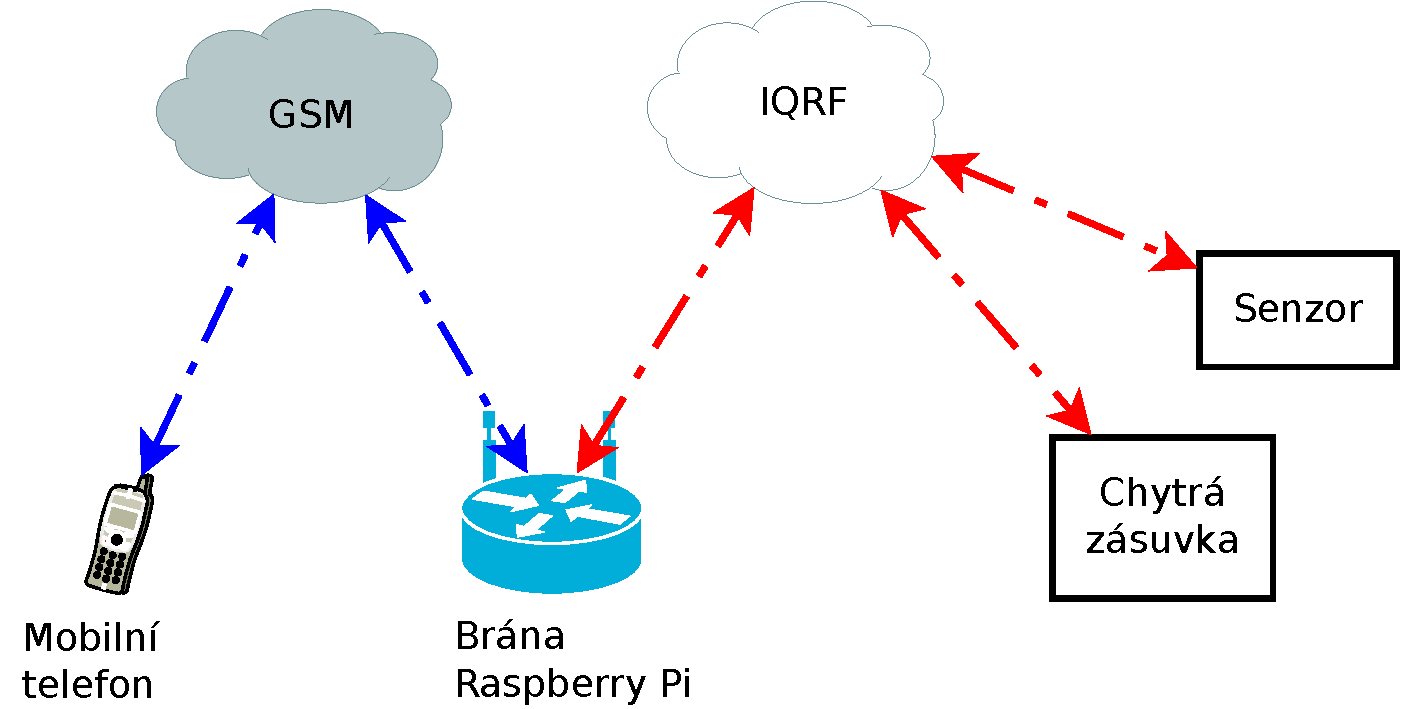
\includegraphics[width = \textwidth]{../img/blokove-schema/komunikace.pdf}
  \end{center}
\end{frame}


%\section{Bloková schémata}
%
%\begin{frame}{Bloková schémata}
%  \begin{center}
%    \minipage{0.50\textwidth}
%      \begin{figure}
%        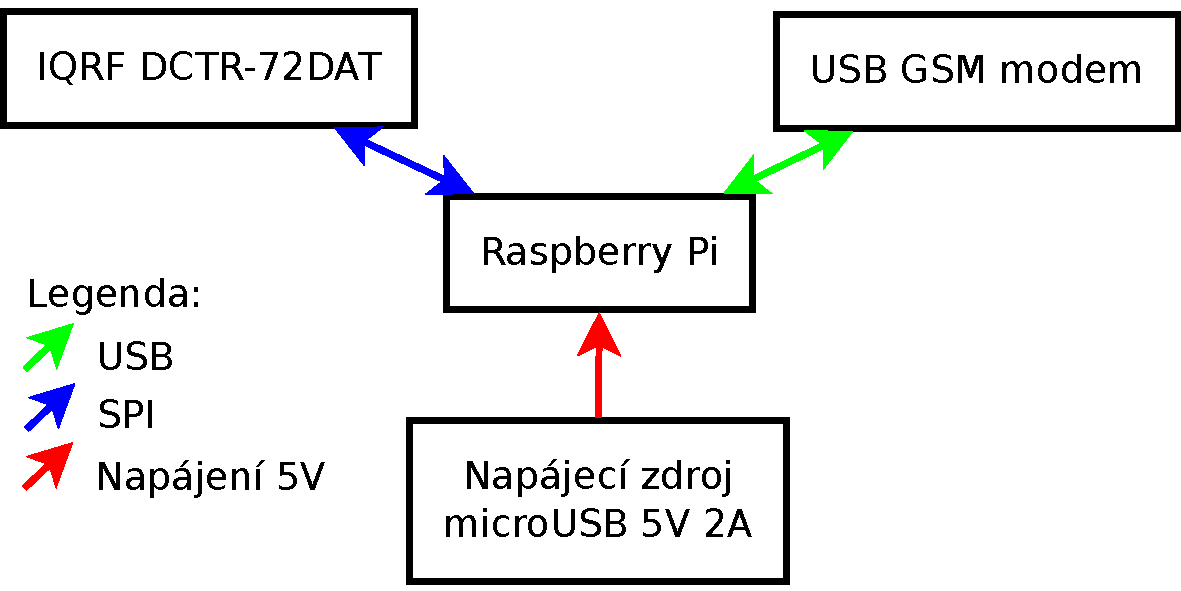
\includegraphics[width = \textwidth]{../img/blokove-schema/brana.pdf}
%        \caption{Brána}
%      \end{figure}
%    \endminipage
%    \minipage{0.50\textwidth}
%      \begin{figure}
%        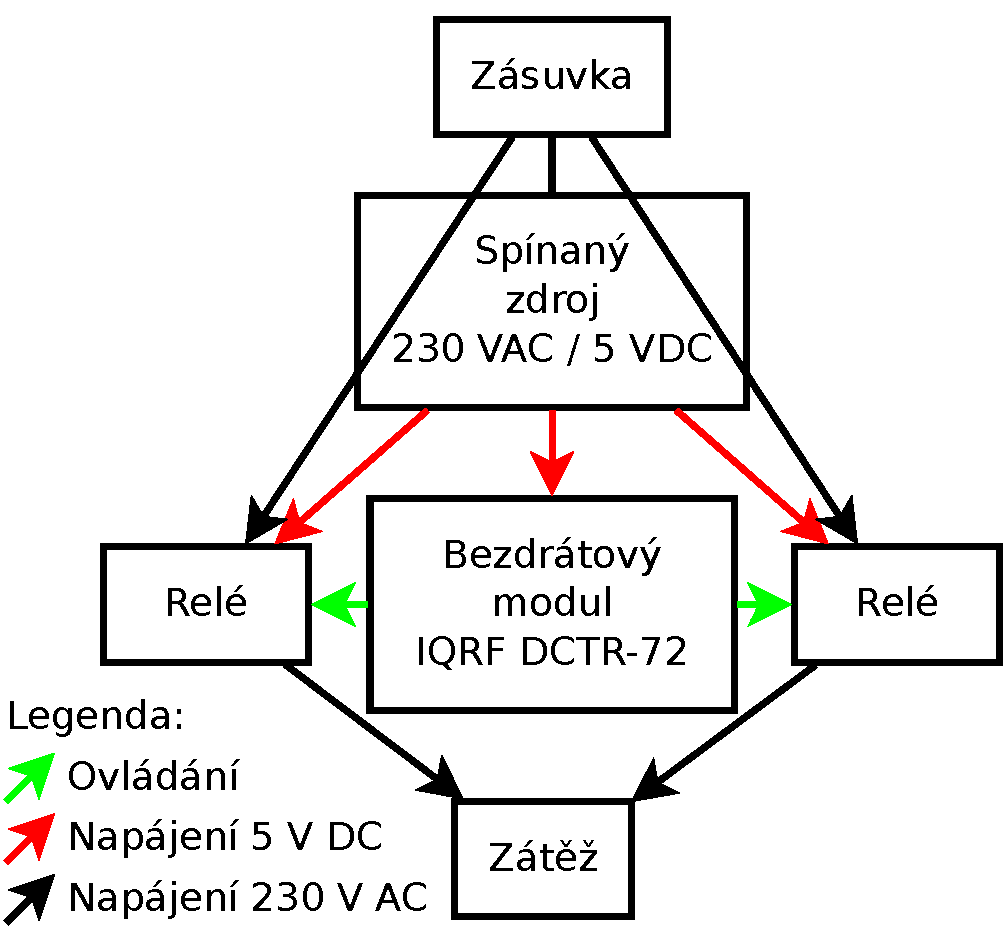
\includegraphics[width = \textwidth]{../img/blokove-schema/zasuvka.pdf}
%        \caption{Chytrá zásuvka}
%      \end{figure}
%    \endminipage
%  \end{center}
%\end{frame}

\section{Fotografie}

\begin{frame}{Fotografie}
  \begin{center}
    \minipage{0.50\textwidth}
      \begin{figure}
        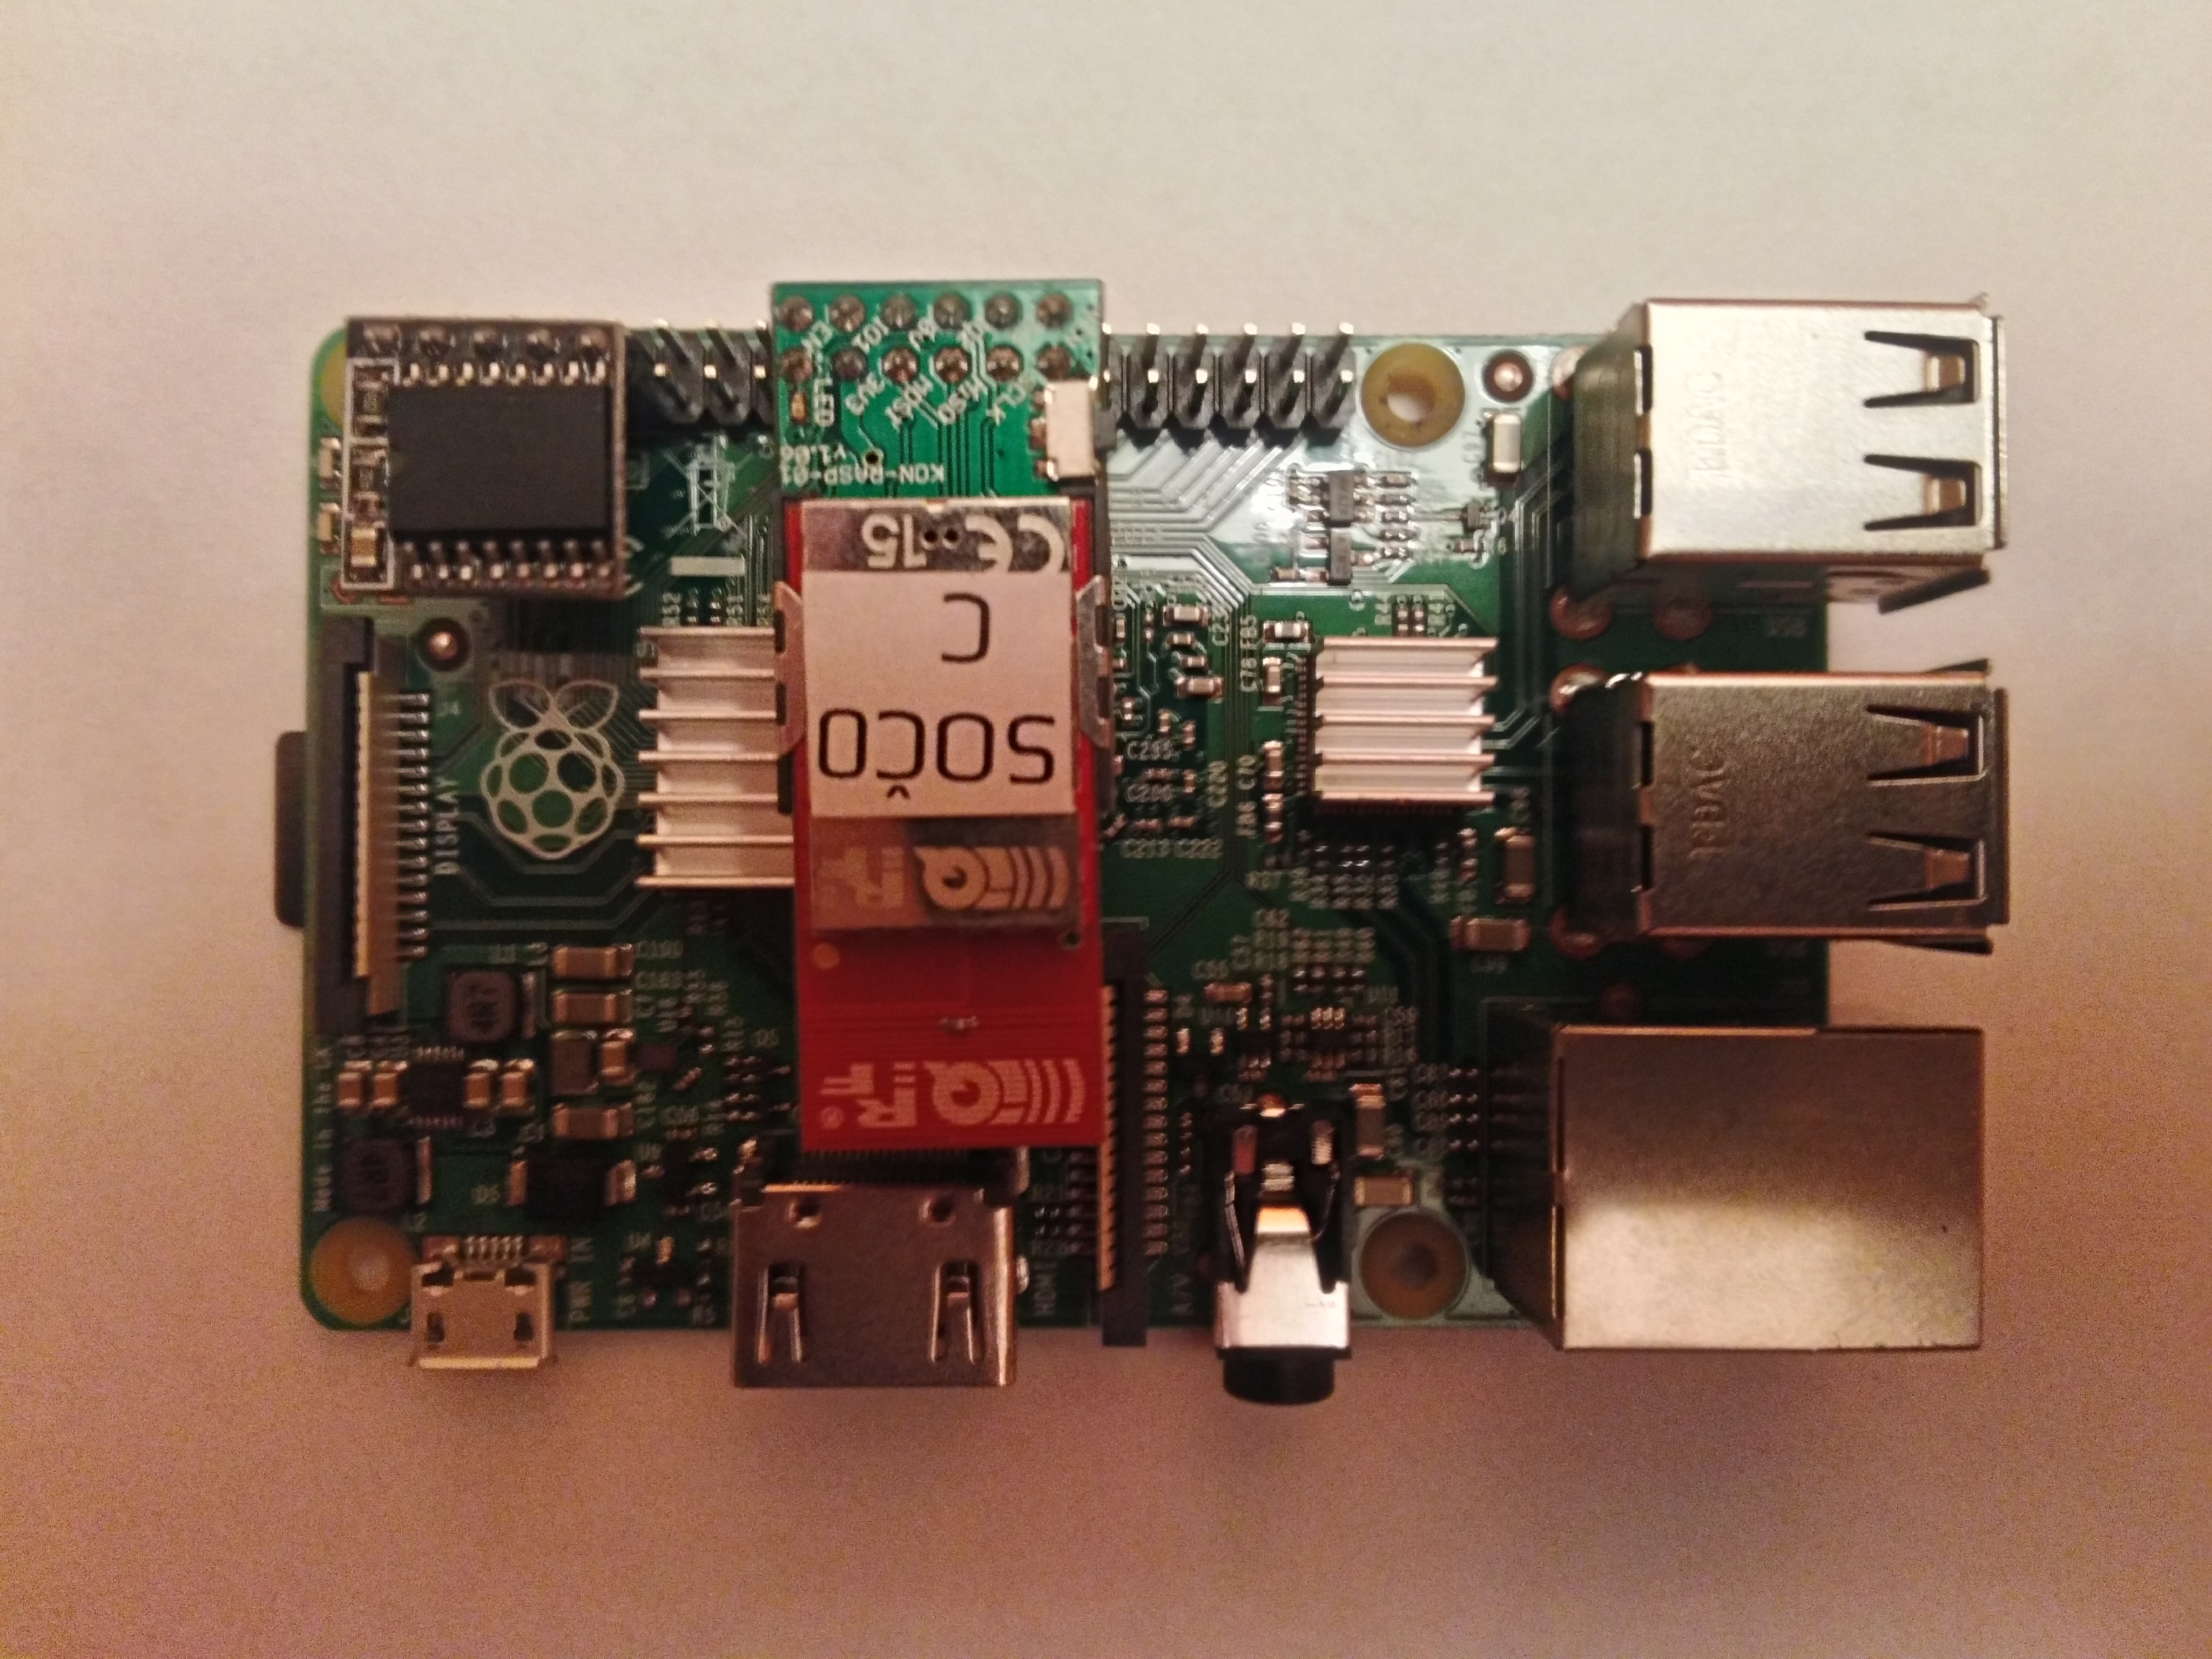
\includegraphics[width = \textwidth]{../img/foto/brana.jpg}
        \caption{Brána}
      \end{figure}
    \endminipage
    \minipage{0.50\textwidth}
      \begin{figure}
        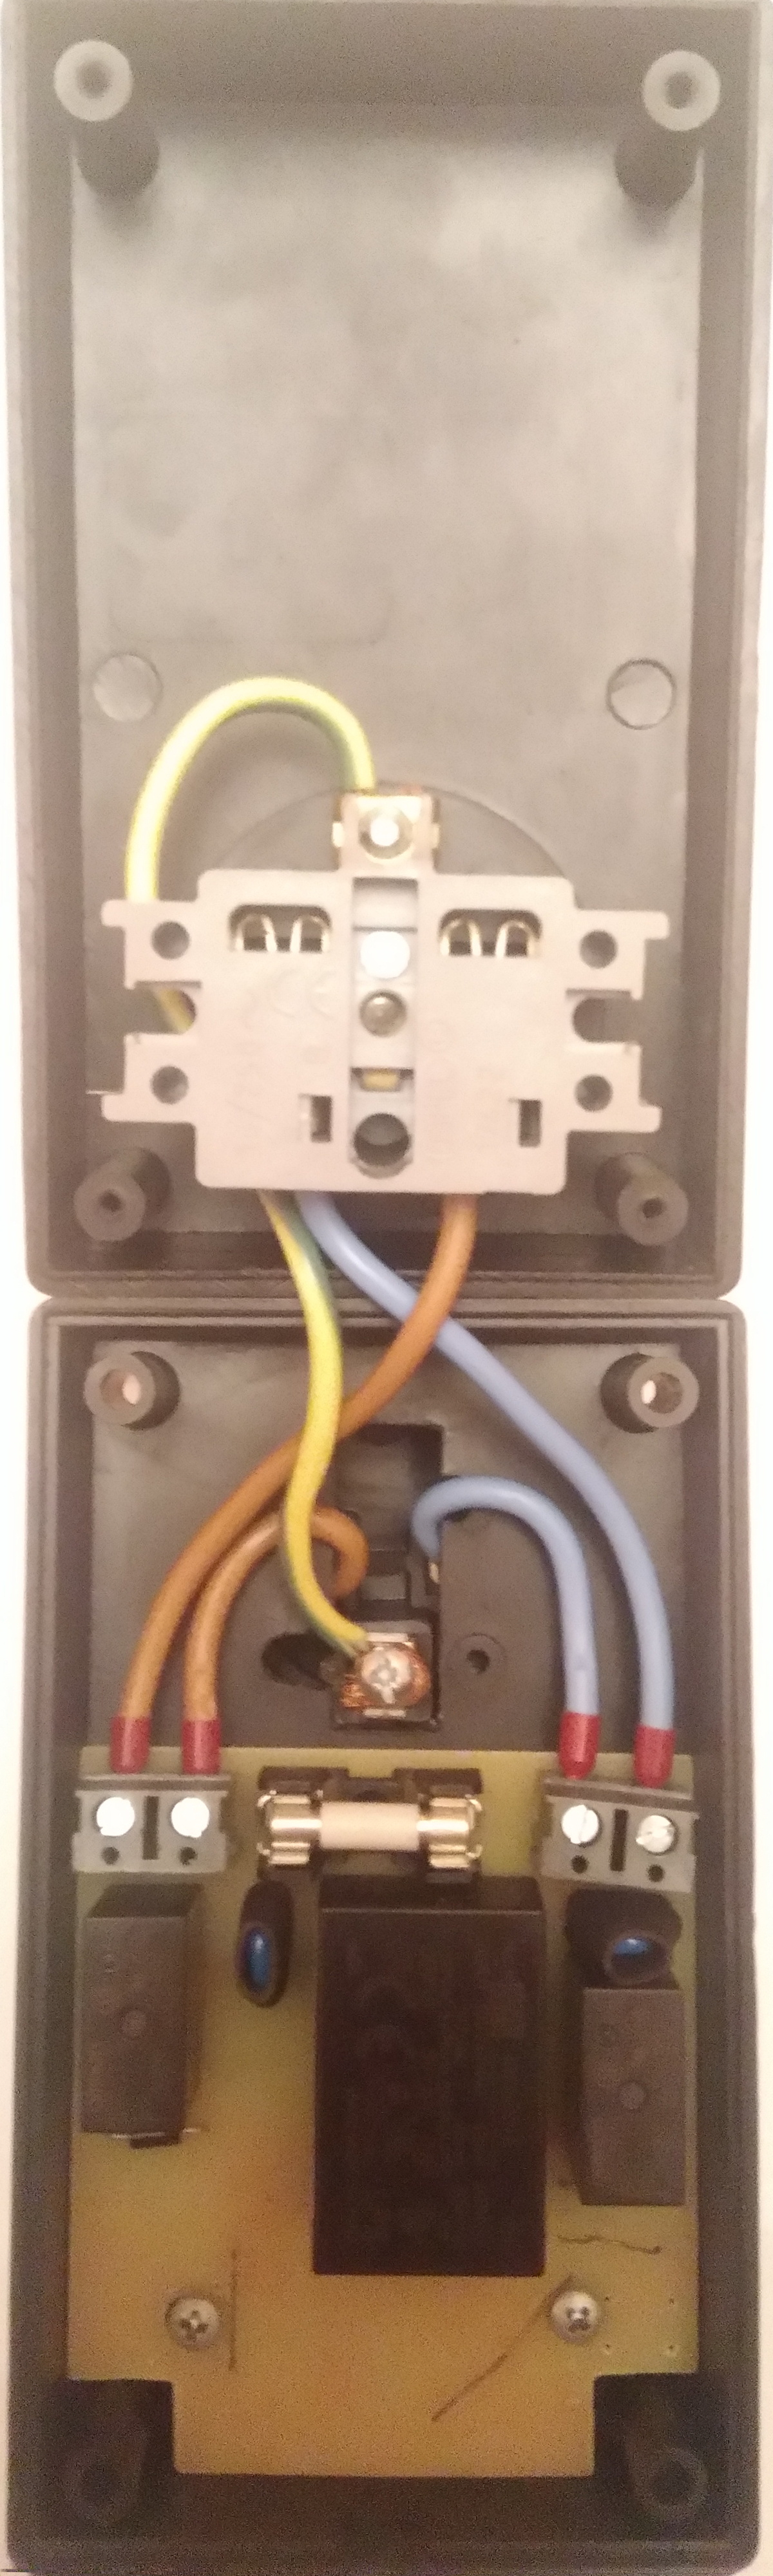
\includegraphics[width = 0.33\textwidth]{../img/foto/zasuvka.jpg}
        \caption{Chytrá zásuvka}
      \end{figure}
    \endminipage
  \end{center}
\end{frame}

\section{Výhody a nevýhody řešení}

\begin{frame}{Výhody a nevýhody řešení}
  \begin{exampleblock}{Výhody}
    \begin{itemize}
      \item Projekt je open-source.
      \item Chytrá zásuvka je provozně bezpečnější než většina konkurenčních zařízení, protože spíná obě zdířky zásuvky.
      \item Díky univerzálnosti a stavebnicovému řešení řešení lze systém dobře rozšiřovat i o další funkce.
    \end{itemize}
  \end{exampleblock}
  \begin{alertblock}{Nevýhody}
    \begin{itemize}
      \item Vyšší cena.
    \end{itemize}
  \end{alertblock}
\end{frame}

\section{Živá ukázka}
\begin{frame}{Živá ukázka}
  \begin{center}
    \huge{\textit{Pravděpodobně} živá ukázka} \\
    \vspace{8mm}
    
\includegraphics[width = 0.33\textwidth]{../img/kocka.png}
    \vspace{8mm}
  \end{center}
  \small{Autor obrázku: Ketrina Yim (draguunthor.deviantart.com)}
\end{frame}

\section{Cíle do budoucna}

\begin{frame}{Cíle do budoucna}
  \begin{itemize}
    \item Doplnění měření spotřeby připojeného spotřebiče.
    \item Doplnění senzorů (např. pro měření teploty, vlhkosti).
    \item Doplnění možnosti ovládat zařízení přes Internet.
    \item Vytvoření mobilní aplikace pro Android, která by zjednodušila ovládání.
  \end{itemize}
\end{frame}

\begin{frame}
  \begin{center}
    \huge{Děkuji za pozornost.} \\[8mm]
    \large{Dotazy?}
  \end{center}
  \vspace{32mm}
  Zdroje obrázků:
  \begin{itemize}
    \item[] \hspace{-5mm} \tiny{\textbf{Schrödingerova kočka:} \url{http://draguunthor.deviantart.com/art/Schrodinger-s-Cat-163302750}}
  \end{itemize}
\end{frame}

\end{document}